\documentclass[11pt, a4paper]{article}

\usepackage{fdsymbol}
\usepackage{subfigure}
\usepackage{float}
\usepackage{graphicx}
\usepackage[extrafootnotefeatures]{xepersian}
\settextfont[Scale=1 ,Path=fonts/, BoldFont={Yas Bold .ttf}, BoldFeatures={Scale = 1.1}]{Yas.ttf}
\newcommand{\mm}{\vspace{1mm}}


\title{گزارش تمرین کامپیوتری اول
	\\
	 درس معماری کامپیوتر پیشرفته}
\author{ امیررضا غلامی\mm \\
	شماره دانشجویی : 810103196 \\
	\\
	پارسا حداد منفرد \\
	شماره دانشجویی : 810103103
}
\date{\today}


\begin{document}
	\maketitle
	\vspace{15cm}
	\tableofcontents
	
	%%%%%%%%%%%%%%%%%%%%%%%%%%%%%%%%%%%%%%%%%
	\pagebreak


	\section{پیاده سازی 
		\lr{single cycle}}
		شماتیک پیاده سازی 
		\lr{single cycle}
		به صورت زیر است.
		\begin{figure}[H]
			\begin{center}
				\includegraphics[width=10cm]{Photos/single_cycle.jpg}
			\end{center}
			\caption{شماتیک پیاده سازی 
			\lr{single cycle}
			}
			\label{single_cycle}
		\end{figure}
	

		
	\subsection{برنامه تست}
	برنامه پیدا کردن بزرگترین عنصر بین 10 عنصر داخل حافظه داده در شکل (
	\ref{test_asm}
	)
	به تصویر کشیده شده است. 
	\begin{figure}[H]
		\begin{center}
			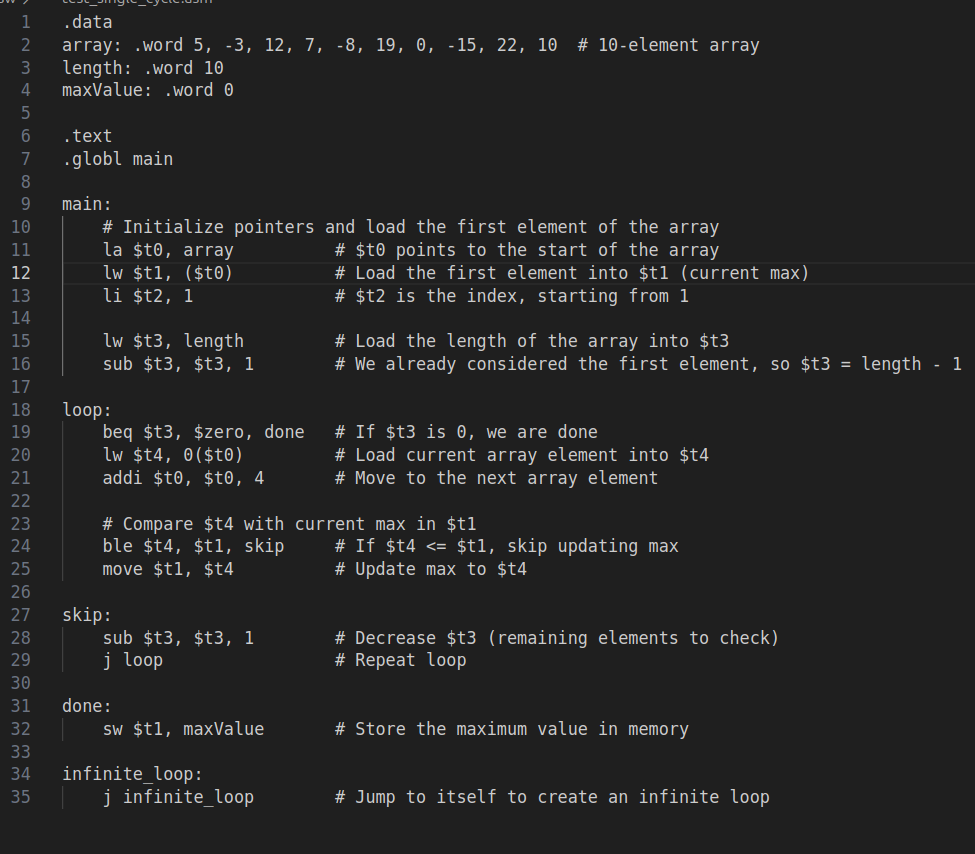
\includegraphics[width=10cm]{Photos/1.png}
		\end{center}
		\caption{برنامه اسمبلی تست}
		\label{test_asm}
	\end{figure}
	
	برنامه اسمبلی را به زبان ماشین (باینری) تبدیل می کنیم
	\begin{figure}[H]
		\begin{center}
			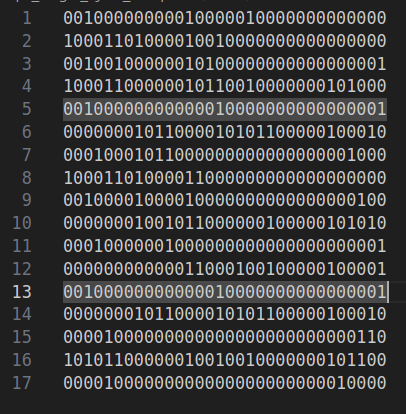
\includegraphics[width=7cm]{Photos/2.png}
		\end{center}
		\caption{دستورات برنامه تست به صورت باینری}
		\label{Inst_Mem}
	\end{figure}
	
	\begin{figure}[H]
		\begin{center}
			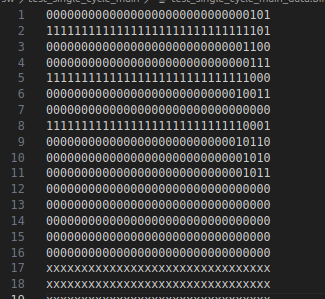
\includegraphics[width=7cm]{Photos/3.png}
		\end{center}
		\caption{داده های برنامه تست به صورت باینری در حافظه داده}
		\label{Data_Mem}
	\end{figure}
	
	
		
	علاوه بر تست فوق، تست دیگری مبنی بر بررسی تمام دستورات زده شده انجام شده است. دستورات NOP به این دلیل است که این تست برای پایپ لاین هم به کار برده شود.
	
	\begin{figure}[H]
		\begin{center}
			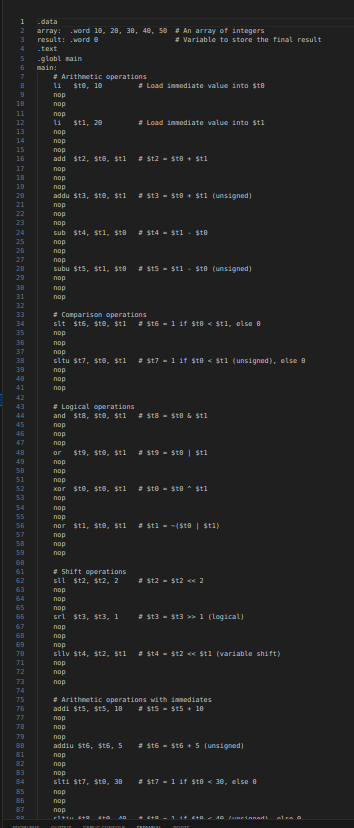
\includegraphics[width=7cm]{Photos/11.png}
		\end{center}
		\caption{تست دوم پایپ لاین}
		\label{mips2_pipeline}
	\end{figure}
	
	
	\subsection{نتایج شبیه سازی}
	
	\begin{figure}[H]
		\begin{center}
			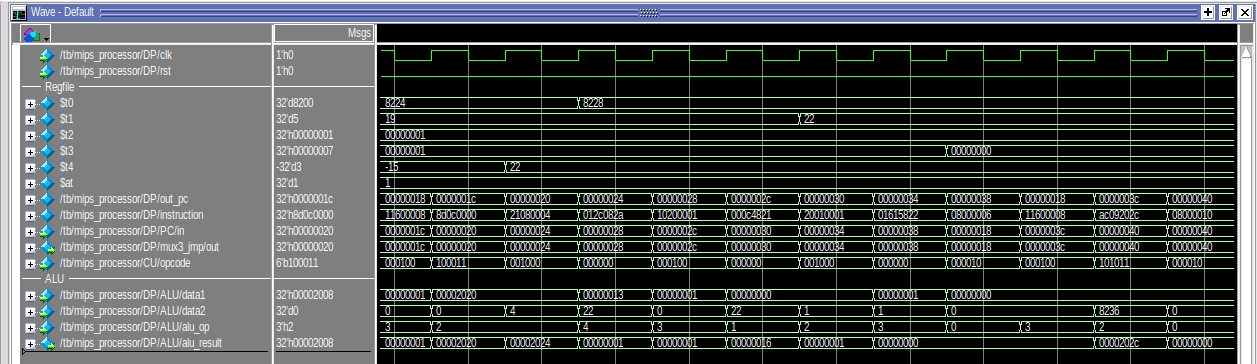
\includegraphics[width=10cm, height=5cm]{Photos/5.png}
			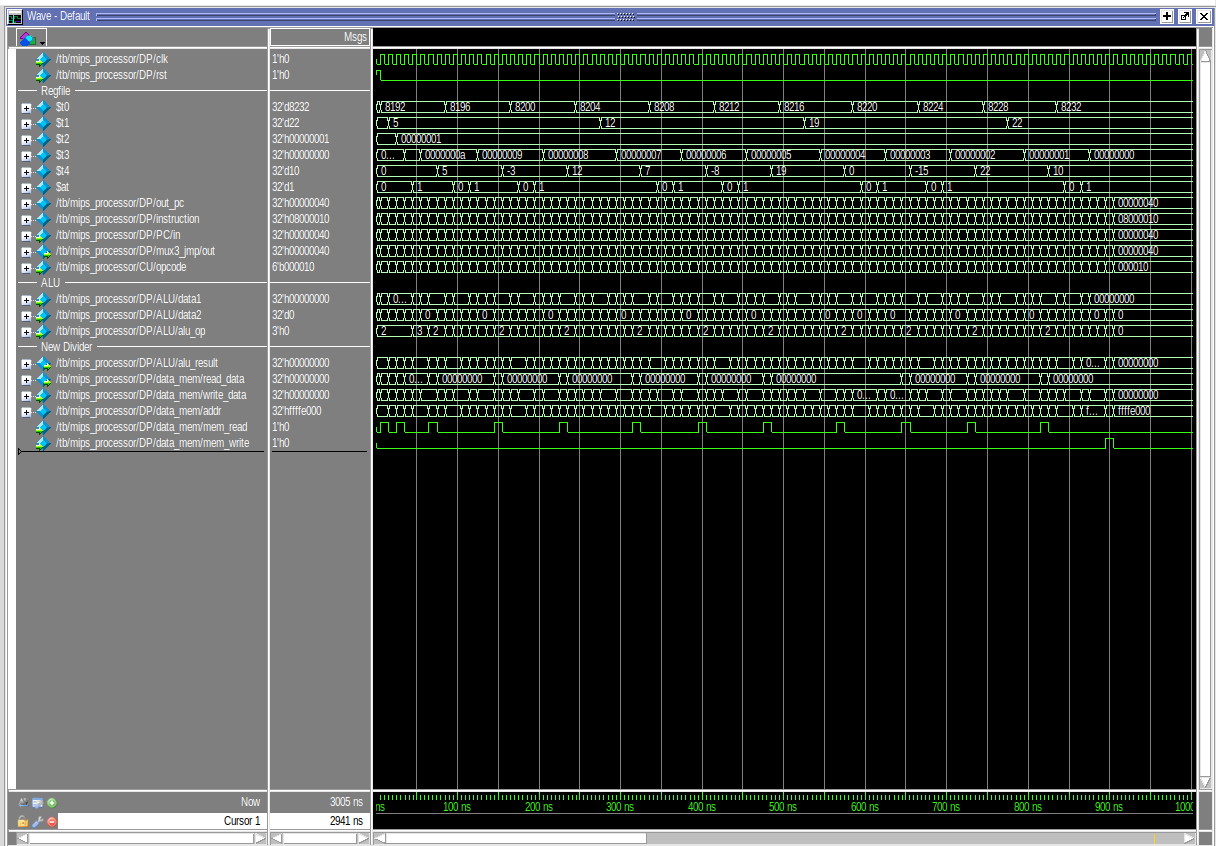
\includegraphics[width=10cm, height=5cm]{Photos/6.png}
		\end{center}
		\caption{شبیه سازی 
		\lr{single cycle}
		}
		\label{Single_cycle_sim}
	\end{figure}
	
	\begin{figure}[H]
		\begin{center}
			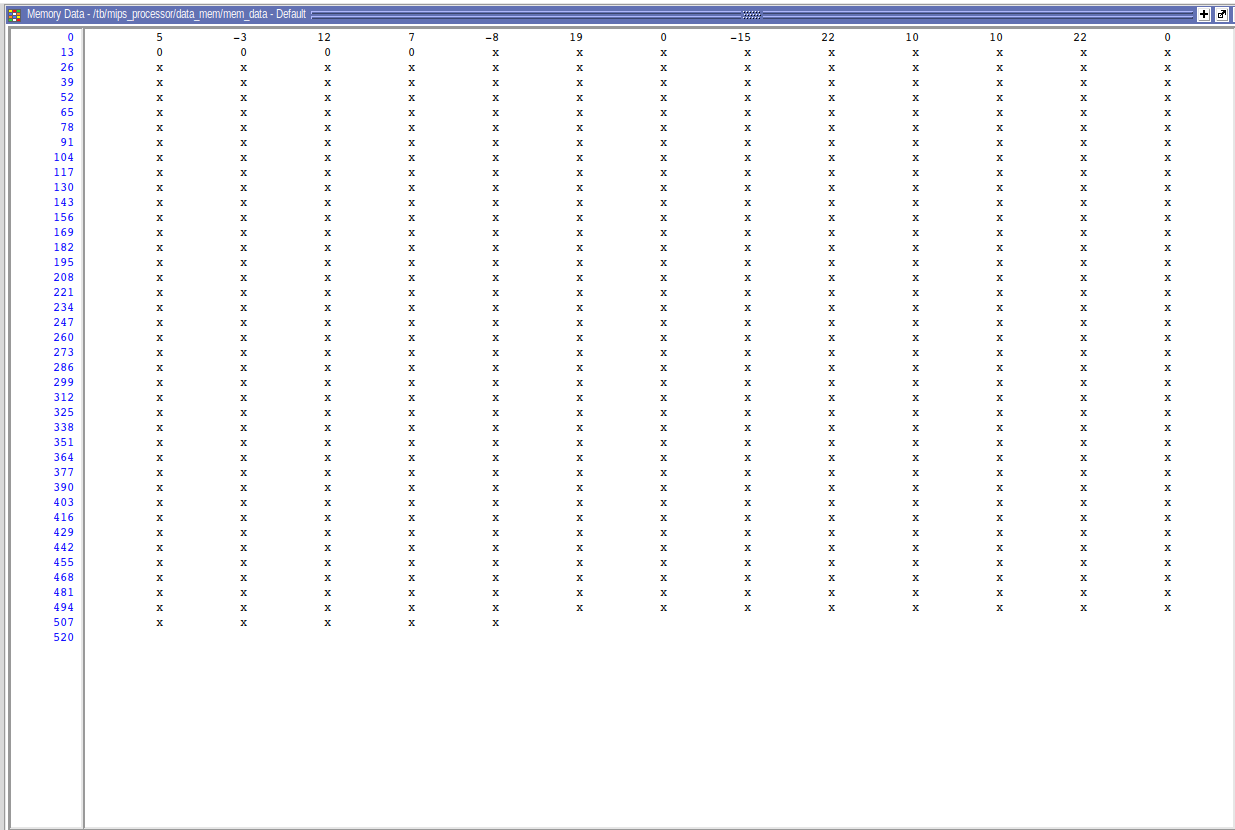
\includegraphics[width=7cm]{Photos/9.png}
		\end{center}
		\caption{حافظه داده در انتهای شبیه سازی 
		\lr{single cycle}
		}
		\label{Single_cycle_data_mem}
	\end{figure}
	
	\begin{figure}[H]
		\begin{center}
			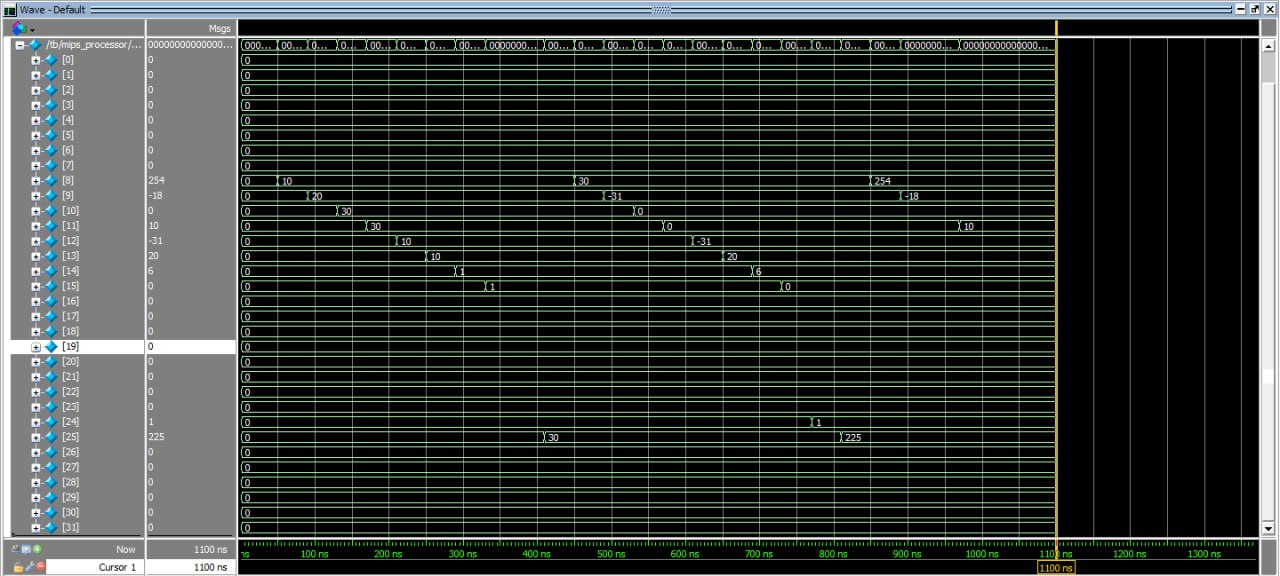
\includegraphics[width=7cm]{Photos/10.jpg}
		\end{center}
		\caption{ نتایج شبیه سازی تست دوم}
		\label{mips2_single_cycle}
	\end{figure}
	
	
	\section{پیاده سازی پایپ لاین}
	
	\begin{figure}[H]
		\begin{center}
			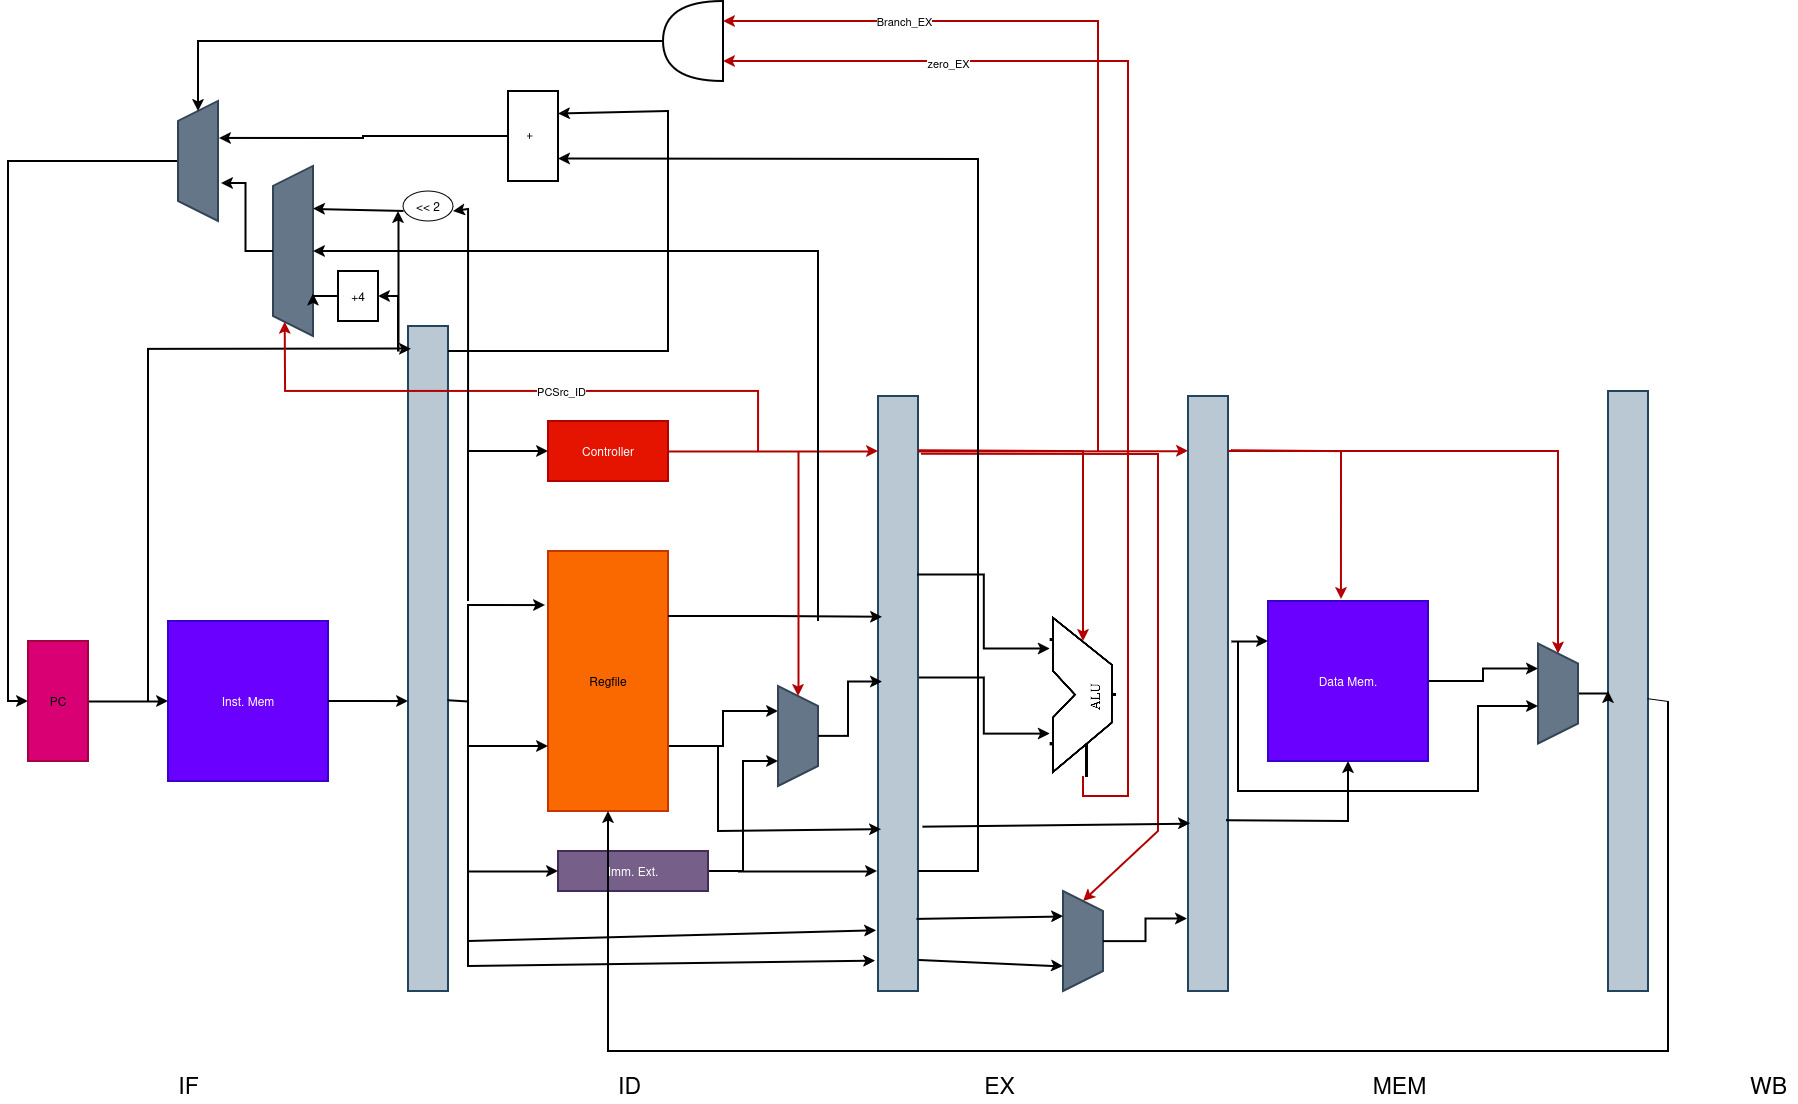
\includegraphics[width=10cm]{Photos/Pipeline_Figure.jpg}
		\end{center}
		\caption{شماتیک مسیرداده پایپ لاین}
		\label{Pipeline_schamitic}
	\end{figure}
 

	\subsection{برنامه تست پایپ لاین}
	برنامه اول تست پایپ لاین همان برنامه تست 
	\lr{single cycle}
	است با این تفاوت که بین تمام دو دستور، سه دستور 
	\lr{NOP}
	قرار داده شده است که از مخاطرات جلوگیری شود که در نتیحه این تغییر باید دستورات 
	\lr{Branch} 
	و
	\lr{Jump}
	تغییر کنند و درست شوند. 
	\begin{figure}[H]
		\begin{center}
			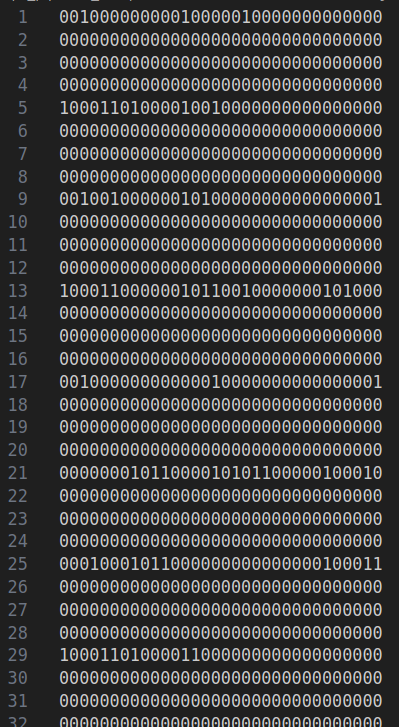
\includegraphics[width=7cm]{Photos/4.png}
		\end{center}
		\caption{حافظه دستورات در پایپ لاین}
		\label{Pipeline_inst_test}
	\end{figure}
	

	
	
	
	\subsection{نتایج شبیه سازی}
	
	\begin{figure}[H]
		\begin{center}
			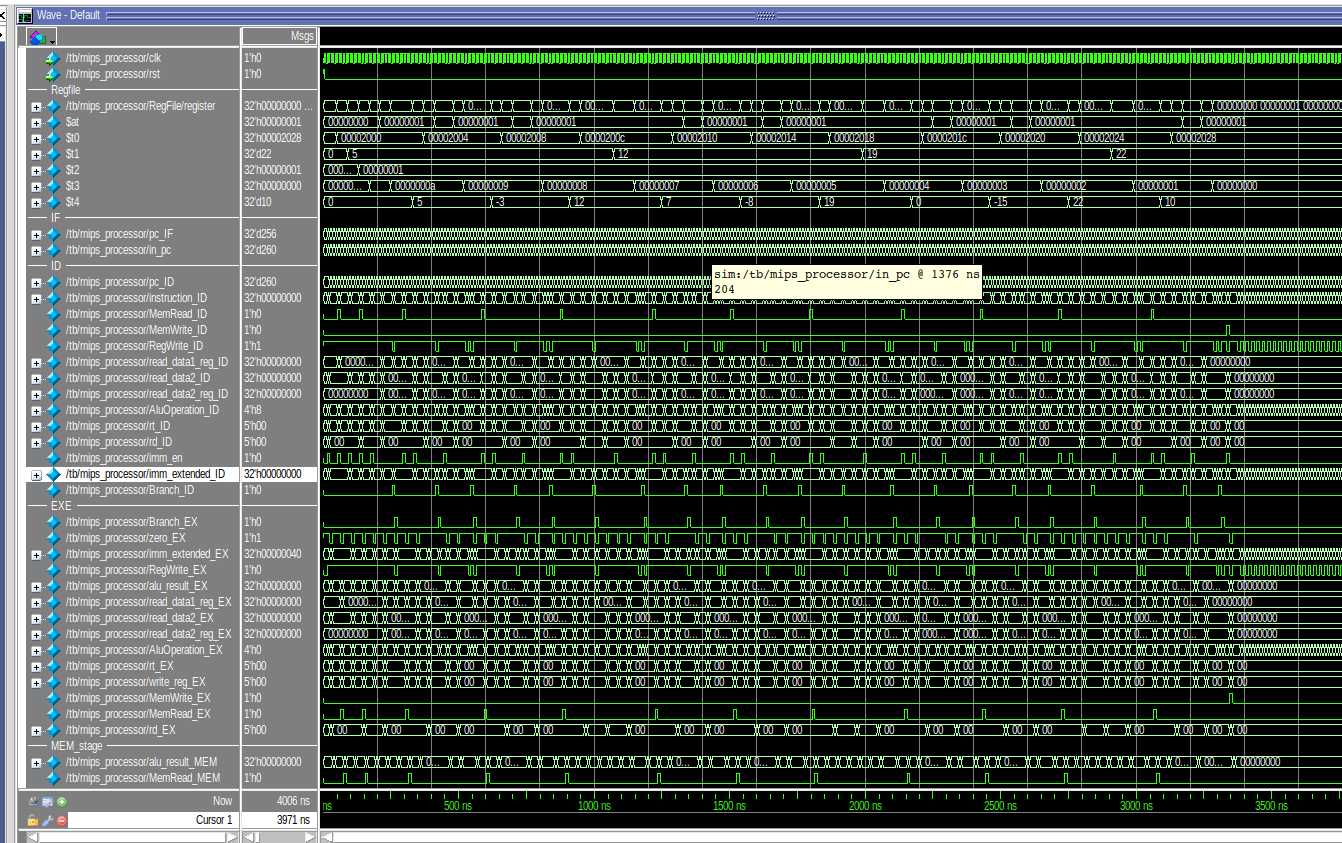
\includegraphics[width=10cm]{Photos/7.png}
			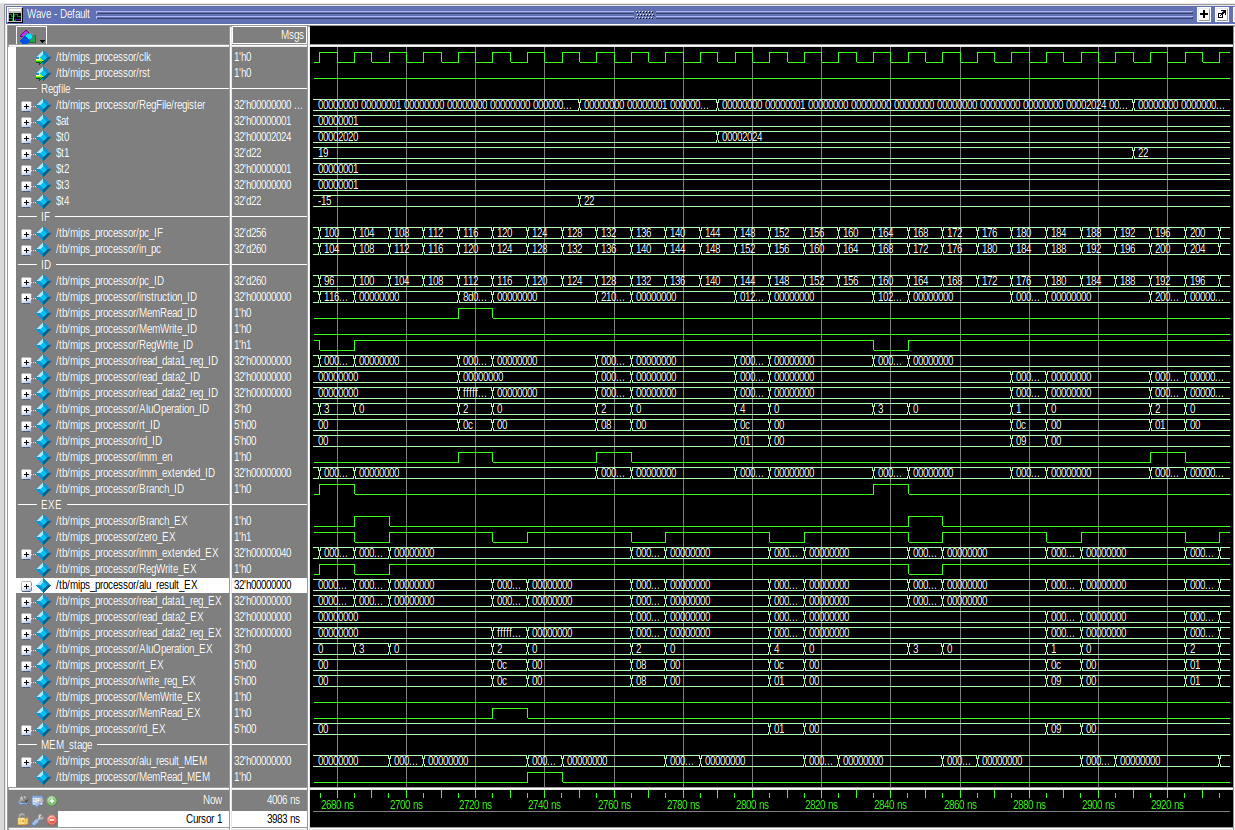
\includegraphics[width=10cm]{Photos/8.png}
		\end{center}
		\caption{شبیه سازی پایپ لاین}
		\label{Pipeline_sim}
	\end{figure}
	
	\begin{figure}[H]
		\begin{center}
			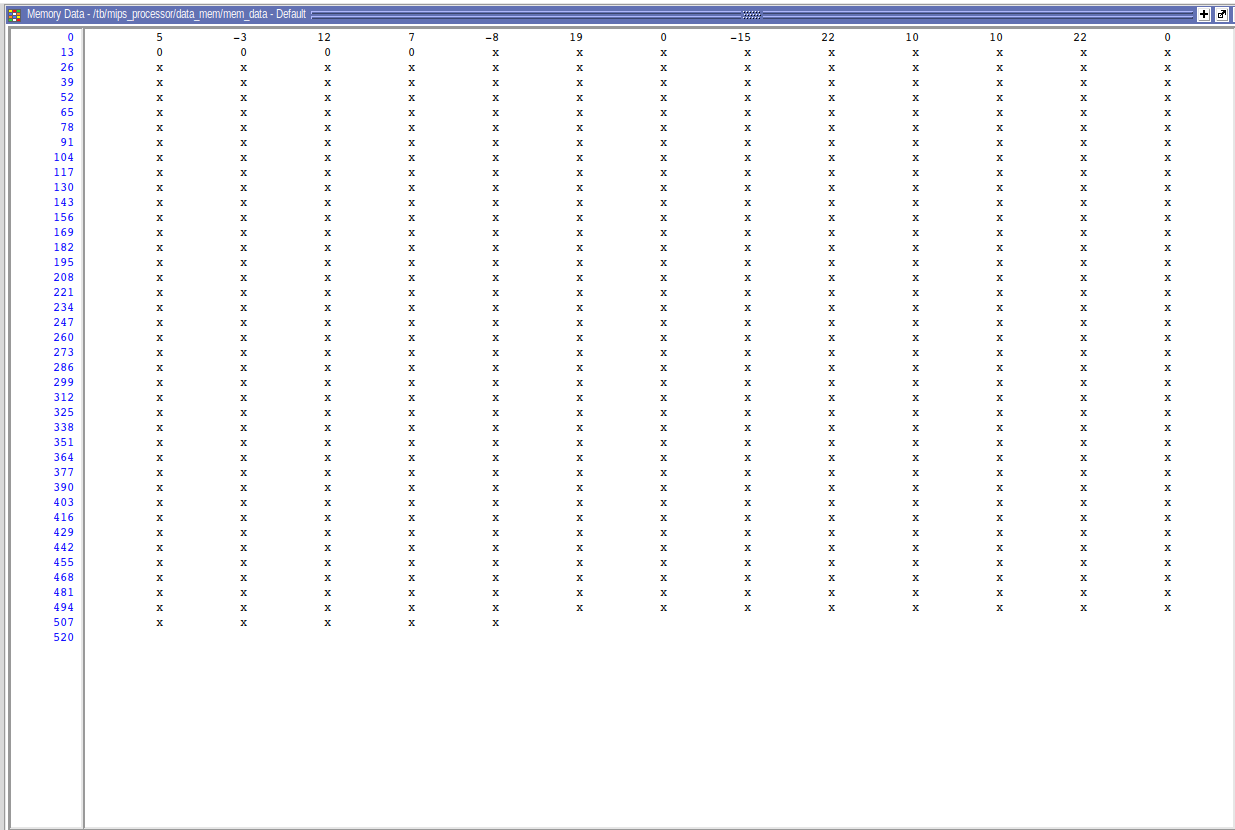
\includegraphics[width=7cm]{Photos/9.png}
		\end{center}
		\caption{حافظه داده در انتهای شبیه سازی پایپ لاین}
		\label{Pipeline_data_mem}
	\end{figure}
	
	
نتایج شبیه سازی تست دوم که تست تمام دستورات است به شرح زیر است:
	\begin{figure}[H]
		\begin{center}
			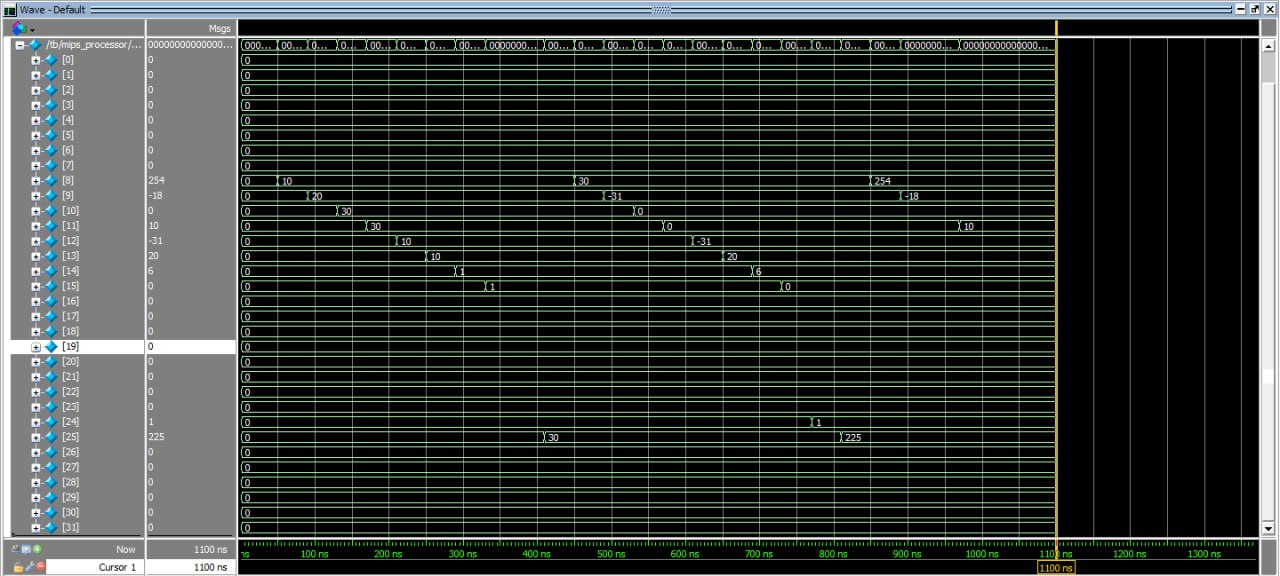
\includegraphics[width=7cm]{Photos/10.jpg}
		\end{center}
		\caption{نتایج شبیه سازی تست دوم پایپ لاین}
		\label{mips2_pipeline_sim}
	\end{figure}
	
\end{document}